\documentclass{article}
\usepackage{tikz}
\usetikzlibrary{arrows.meta}

\begin{document}

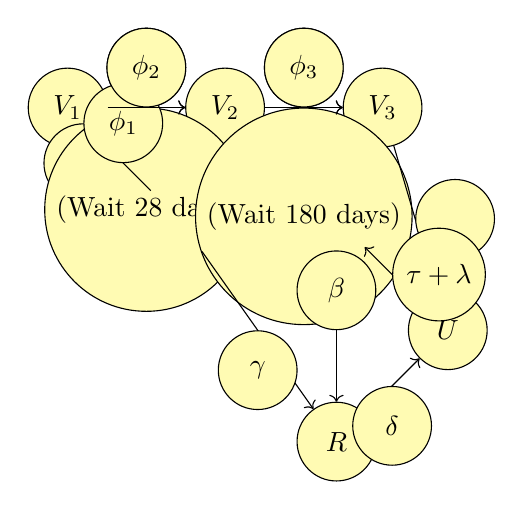
\begin{tikzpicture}[node distance=2cm, auto]
    \tikzstyle{every node}=[draw, circle, fill=yellow!30, minimum size=1cm]

    \node (S) {$S$};
    \node (E) [right of=S] {$E$};
    \node (U) [below right of=E] {$U$};
    \node (R) [below left of=U] {$R$};
    \node (V1) [above left of=S] {$V_1$};
    \node (V2) [right of=V1] {$V_2$};
    \node (V3) [right of=V2] {$V_3$};

    \path[->]
        (S) edge node [left] {$\alpha_1$} (V1)
        (V1) edge node [above] {$\alpha_2$} node [pos=0.5, below] {(Wait 28 days)} (V2)
        (V2) edge node [above] {$\alpha_3$} node [pos=0.5, below] {(Wait 180 days)} (V3)
        (V3) edge node [right] {} (U)
        (U) edge node [right] {$\tau + \lambda$} (E)
        (E) edge node [above] {$\beta$} (R)
        (R) edge node [below] {$\delta$} (U)
        (S) edge node [above] {$\phi_1$} (V1)
        (V1) edge node [above] {$\phi_2$} (V2)
        (V2) edge node [above] {$\phi_3$} (V3)
        (S) edge node [below] {$\gamma$} (R);
\end{tikzpicture}

\captionof{figure}{The SIRV Compartmental Model for COVID-19 disease dynamics (similar to the one in Abou-Ismail et al \cite{Abou-Ismail2020}), consisting Susceptible ($S$), Exposed ($E$), Quarantined ($U$), Recovered ($R$), and Vaccinated ($V$) compartments. Three doses of vaccination are assumed, the second and the third being administered 28 and 208 days after the first. The transmission rate is $\beta$, recovery rate is $\delta$, the rate of becoming susceptible after disease is $\gamma$, the vaccination rates are $\alpha_i$ for $i^{th}$ vaccination, calculated as a proportion of people who took the previous vaccine, and the rate of vaccination immunity wearing off from $i^{th}$ vaccination is $\phi_i$.}
\label{fig:SIRV_model}

\end{document}